%%%%%%%%%%%%%%%%%%%%%%%%%%%%%%%%%%%%%%%%%
% Masters/Doctoral Thesis 
% LaTeX Template
% Version 2.5 (27/8/17)
%
% This template was downloaded from:
% http://www.LaTeXTemplates.com
%
% Version 2.x major modifications by:
% Vel (vel@latextemplates.com)
%
% This template is based on a template by:
% Steve Gunn (http://users.ecs.soton.ac.uk/srg/softwaretools/document/templates/)
% Sunil Patel (http://www.sunilpatel.co.uk/thesis-template/)
%
% Template license:
% CC BY-NC-SA 3.0 (http://creativecommons.org/licenses/by-nc-sa/3.0/)
%
%%%%%%%%%%%%%%%%%%%%%%%%%%%%%%%%%%%%%%%%%

%----------------------------------------------------------------------------------------
%	PACKAGES AND OTHER DOCUMENT CONFIGURATIONS
%----------------------------------------------------------------------------------------

\documentclass[
11pt, % The default document font size, options: 10pt, 11pt, 12pt
%oneside, % Two side (alternating margins) for binding by default, uncomment to switch to one side
english, % ngerman for German
singlespacing, % Single line spacing, alternatives: onehalfspacing or doublespacing
%draft, % Uncomment to enable draft mode (no pictures, no links, overfull hboxes indicated)
%nolistspacing, % If the document is onehalfspacing or doublespacing, uncomment this to set spacing in lists to single
%liststotoc, % Uncomment to add the list of figures/tables/etc to the table of contents
%toctotoc, % Uncomment to add the main table of contents to the table of contents
%parskip, % Uncomment to add space between paragraphs
%nohyperref, % Uncomment to not load the hyperref package
headsepline, % Uncomment to get a line under the header
%chapterinoneline, % Uncomment to place the chapter title next to the number on one line
%consistentlayout, % Uncomment to change the layout of the declaration, abstract and acknowledgements pages to match the default layout
]{MastersDoctoralThesis} % The class file specifying the document structure

\usepackage[utf8]{inputenc} % Required for inputting international characters
\usepackage[T1]{fontenc} % Output font encoding for international characters

\usepackage{mathpazo} % Use the Palatino font by default

\usepackage[backend=bibtex,style=authoryear,natbib=true]{biblatex} % Use the bibtex backend with the authoryear citation style (which resembles APA)

\addbibresource{example.bib} % The filename of the bibliography

\usepackage[autostyle=true]{csquotes} % Required to generate language-dependent quotes in the bibliography

%----------------------------------------------------------------------------------------
%	MARGIN SETTINGS
%----------------------------------------------------------------------------------------

\geometry{
	paper=a4paper, % Change to letterpaper for US letter
	inner=2.5cm, % Inner margin
	outer=3.8cm, % Outer margin
	bindingoffset=.5cm, % Binding offset
	top=1.5cm, % Top margin
	bottom=1.5cm, % Bottom margin
	%showframe, % Uncomment to show how the type block is set on the page
}

%----------------------------------------------------------------------------------------
%	THESIS INFORMATION
%----------------------------------------------------------------------------------------

\thesistitle{Thesis Title} % Your thesis title, this is used in the title and abstract, print it elsewhere with \ttitle
\supervisor{Dr. James \textsc{Smith}} % Your supervisor's name, this is used in the title page, print it elsewhere with \supname
\examiner{} % Your examiner's name, this is not currently used anywhere in the template, print it elsewhere with \examname
\degree{Doctor of Philosophy} % Your degree name, this is used in the title page and abstract, print it elsewhere with \degreename
\author{John \textsc{Smith}} % Your name, this is used in the title page and abstract, print it elsewhere with \authorname
\addresses{} % Your address, this is not currently used anywhere in the template, print it elsewhere with \addressname

\subject{Biological Sciences} % Your subject area, this is not currently used anywhere in the template, print it elsewhere with \subjectname
\keywords{} % Keywords for your thesis, this is not currently used anywhere in the template, print it elsewhere with \keywordnames
\university{\href{http://www.university.com}{University Name}} % Your university's name and URL, this is used in the title page and abstract, print it elsewhere with \univname
\department{\href{http://department.university.com}{Department or School Name}} % Your department's name and URL, this is used in the title page and abstract, print it elsewhere with \deptname
\group{\href{http://researchgroup.university.com}{Research Group Name}} % Your research group's name and URL, this is used in the title page, print it elsewhere with \groupname
\faculty{\href{http://faculty.university.com}{Faculty Name}} % Your faculty's name and URL, this is used in the title page and abstract, print it elsewhere with \facname

\AtBeginDocument{
\hypersetup{pdftitle=\ttitle} % Set the PDF's title to your title
\hypersetup{pdfauthor=\authorname} % Set the PDF's author to your name
\hypersetup{pdfkeywords=\keywordnames} % Set the PDF's keywords to your keywords
}

\begin{document}

\frontmatter % Use roman page numbering style (i, ii, iii, iv...) for the pre-content pages

\pagestyle{plain} % Default to the plain heading style until the thesis style is called for the body content

%----------------------------------------------------------------------------------------
%	TITLE PAGE
%----------------------------------------------------------------------------------------

\begin{titlepage}
\begin{center}

\vspace*{.06\textheight}
{\scshape\LARGE \univname\par}\vspace{1.5cm} % University name
\textsc{\Large Doctoral Thesis}\\[0.5cm] % Thesis type

\HRule \\[0.4cm] % Horizontal line
{\huge \bfseries \ttitle\par}\vspace{0.4cm} % Thesis title
\HRule \\[1.5cm] % Horizontal line
 
\begin{minipage}[t]{0.4\textwidth}
\begin{flushleft} \large
\emph{Author:}\\
\href{http://www.johnsmith.com}{\authorname} % Author name - remove the \href bracket to remove the link
\end{flushleft}
\end{minipage}
\begin{minipage}[t]{0.4\textwidth}
\begin{flushright} \large
\emph{Supervisor:} \\
\href{http://www.jamessmith.com}{\supname} % Supervisor name - remove the \href bracket to remove the link  
\end{flushright}
\end{minipage}\\[3cm]
 
\vfill

\large \textit{A thesis submitted in fulfillment of the requirements\\ for the degree of \degreename}\\[0.3cm] % University requirement text
\textit{in the}\\[0.4cm]
\groupname\\\deptname\\[2cm] % Research group name and department name
 
\vfill

{\large \today}\\[4cm] % Date
%\includegraphics{Logo} % University/department logo - uncomment to place it
 
\vfill
\end{center}
\end{titlepage}

%----------------------------------------------------------------------------------------
%	DECLARATION PAGE
%----------------------------------------------------------------------------------------

\begin{declaration}
\addchaptertocentry{\authorshipname} % Add the declaration to the table of contents
\noindent I, \authorname, declare that this thesis titled, \enquote{\ttitle} and the work presented in it are my own. I confirm that:

\begin{itemize} 
\item This work was done wholly or mainly while in candidature for a research degree at this University.
\item Where any part of this thesis has previously been submitted for a degree or any other qualification at this University or any other institution, this has been clearly stated.
\item Where I have consulted the published work of others, this is always clearly attributed.
\item Where I have quoted from the work of others, the source is always given. With the exception of such quotations, this thesis is entirely my own work.
\item I have acknowledged all main sources of help.
\item Where the thesis is based on work done by myself jointly with others, I have made clear exactly what was done by others and what I have contributed myself.\\
\end{itemize}
 
\noindent Signed:\\
\rule[0.5em]{25em}{0.5pt} % This prints a line for the signature
 
\noindent Date:\\
\rule[0.5em]{25em}{0.5pt} % This prints a line to write the date
\end{declaration}

\cleardoublepage

%----------------------------------------------------------------------------------------
%	QUOTATION PAGE
%----------------------------------------------------------------------------------------

\vspace*{0.2\textheight}

\noindent\enquote{\itshape Thanks to my solid academic training, today I can write hundreds of words on virtually any topic without possessing a shred of information, which is how I got a good job in journalism.}\bigbreak

\hfill Dave Barry

%----------------------------------------------------------------------------------------
%	ABSTRACT PAGE
%----------------------------------------------------------------------------------------

\begin{abstract}
\addchaptertocentry{\abstractname} % Add the abstract to the table of contents

% TODO: add references to these papers in the abstract
%There exists many deep learning compiler frameworks including: TVM, DeepTools, TensorFlow XLA, DLVM, nGraph, and Glow that all focus optimizing the performance of
%runtime and training of deep learning workloads with the aim of being hardware agnostic for most. Some of these optimizations include parallelization, rescheduling,
%operator fusion, and off chip memory accesses. 
%
%While the OnSRAM paper has demonstrated significant improvements in memory
%efficiency and performance in deep learning accelerators (DLAs) through
%optimized on-chip scratchpad management, it relies on a single monolithic
%scratchpad. In this work, we present a novel approach that builds upon the
%OnSRAM concept by implementing a dynamic scratchpad allocation scheme, enabling
%further optimization and energy savings in DLAs.
%
%However, they largely overlook the potential for inter-node communication and
%data reuse optimization within on-chip memory resources. Our implementation
%addresses this gap by introducing a dynamic scratchpad allocation scheme that
%allows for more fine-grained control over memory resources, further reducing
%energy consumption and latency associated with inter-node data movement.
%
%Our work extends the OnSRAM approach by incorporating a dynamic scratchpad
%allocation scheme, enabling a more flexible and efficient use of on-chip
%memory resources in deep learning accelerators. This advancement has the
%potential to significantly enhance the performance and energy efficiency of
%various deep learning applications
%
%something something about how everyone uses graph compiling into IR or graph level optimizations
%
%inter node chip managemernt

%----------------------------------------------------------------------------------
%----------- Sorta the real section -----------------------------------------------
%----------------------------------------------------------------------------------
The landscape of deep learning compiler frameworks has evolved rapidly with the
development of various tools, such as TVM, deeptools, TensorFlow, DLVM, nGraph,
and Glow. These frameworks offer unique optimizations to address computation
and data movement challenges in deep learning accelerators (DLAs). These
approaches include graph or IR level optimizations related to intra node memory
access optimizations, operator fusion, and various tiling techniques. Despite
their unique approaches, these frameworks primarily concentrate on node level
optimizations that focus on increasing the performance of executing a scheduled
operation in the graph and overlook the potential for inter-node data reuse
optimizations within on-chip memory resources.

OnSRAM, a novel approach, addresses this gap by focusing on internode
scratchpad management in DLAs.

%%% TODO REWRITE THIS ECTIOn
It leverages data locality and temporal data
reuse principles through a hierarchical memory allocation scheme, inter-node
data prefetching mechanism, and dynamic memory reconfiguration mechanism. These
components work together to minimize off-chip memory accesses and efficiently
manage a single monolithic on-chip scratchpad, leading to significant
improvements in energy consumption and latency.

% TODO we can use our work to be used as an extension to existing graph level optimziations frameworks
% and not necessarily have to be a standalone like OnSRAM
In this work, we extend the capabilities of OnSRAM by introducing dynamic
scratchpad allocation for static graph execution models using any number of
scratchpads. This enhancement allows for more fine-grained control over on-chip
memory resources, providing increased flexibility and adaptability to better
accommodate diverse deep learning accelerators and memory access patterns. By
optimizing inter-node data movement and storage across multiple scratchpads,
our approach further reduces energy consumption and latency associated with
inter-node communication.

\end{abstract}

%----------------------------------------------------------------------------------------
%	ACKNOWLEDGEMENTS
%----------------------------------------------------------------------------------------

\begin{acknowledgements}
\addchaptertocentry{\acknowledgementname} % Add the acknowledgements to the table of contents
The acknowledgments and the people to thank go here, don't forget to include your project advisor\ldots
\end{acknowledgements}

%----------------------------------------------------------------------------------------
%	LIST OF CONTENTS/FIGURES/TABLES PAGES
%----------------------------------------------------------------------------------------

\tableofcontents % Prints the main table of contents

\listoffigures % Prints the list of figures

\listoftables % Prints the list of tables

%----------------------------------------------------------------------------------------
%	ABBREVIATIONS
%----------------------------------------------------------------------------------------

\begin{abbreviations}{ll} % Include a list of abbreviations (a table of two columns)

\textbf{LAH} & \textbf{L}ist \textbf{A}bbreviations \textbf{H}ere\\
\textbf{WSF} & \textbf{W}hat (it) \textbf{S}tands \textbf{F}or\\

\end{abbreviations}

%----------------------------------------------------------------------------------------
%	PHYSICAL CONSTANTS/OTHER DEFINITIONS
%----------------------------------------------------------------------------------------

\begin{constants}{lr@{${}={}$}l} % The list of physical constants is a three column table

% The \SI{}{} command is provided by the siunitx package, see its documentation for instructions on how to use it

Speed of Light & $c_{0}$ & \SI{2.99792458e8}{\meter\per\second} (exact)\\
%Constant Name & $Symbol$ & $Constant Value$ with units\\

\end{constants}

%----------------------------------------------------------------------------------------
%	SYMBOLS
%----------------------------------------------------------------------------------------

\begin{symbols}{lll} % Include a list of Symbols (a three column table)

$a$ & distance & \si{\meter} \\
$P$ & power & \si{\watt} (\si{\joule\per\second}) \\
%Symbol & Name & Unit \\

\addlinespace % Gap to separate the Roman symbols from the Greek

$\omega$ & angular frequency & \si{\radian} \\

\end{symbols}

%----------------------------------------------------------------------------------------
%	DEDICATION
%----------------------------------------------------------------------------------------

\dedicatory{For/Dedicated to/To my\ldots} 

%----------------------------------------------------------------------------------------
%	THESIS CONTENT - CHAPTERS
%----------------------------------------------------------------------------------------

\mainmatter % Begin numeric (1,2,3...) page numbering

\pagestyle{thesis} % Return the page headers back to the "thesis" style

% Include the chapters of the thesis as separate files from the Chapters folder
% Uncomment the lines as you write the chapters


\chapter{Background} % Main chapter title

\label{Chapter1} % Change X to a consecutive number; for referencing this chapter elsewhere, use \ref{ChapterX}

%----------------------------------------------------------------------------------------
%	SECTION 1
%----------------------------------------------------------------------------------------

\section{Deep Learning Architectures}

%-----------------------------------
%	SUBSECTION 1
%-----------------------------------
\subsection{Perceptron}

%-----------------------------------
%	SUBSECTION 2
%-----------------------------------
\subsection{CNN}

%-----------------------------------
%	SUBSECTION 3
%-----------------------------------

\subsection{RNN}


%-----------------------------------
%	SUBSECTION 4
%-----------------------------------

\subsection{LSTM}

%----------------------------------------------------------------------------------------
%	SECTION 2
%----------------------------------------------------------------------------------------
\section{Accelerators and Scratchpad Memory}
Deep learning accelerators (DLA) are hardware made specifically to accelerate
common operations needed to run inference or training on DL models. 

\subsection{Existing Scratchpad Memory Management Schemes}

\section{Deep Learning Frameworks}
\subsection{Introduction}
In order to create to run a DL model, a programmer must describe the
architecture, its input and output layers, and the inputs that will be passed
to the model. Beyond these properties, the implementation and challenges
associated with deploying such a model on a DLA or distributed system is
handled by deep learning frameworks. Deep learning frameworks abstract the
implementation and execution details from the programmer such that the
programmer may focus on the model creation only. The abstraction of such
details forces the trade-off of performance and generality as the frameworks
must optimize the same model for runtime and memory efficiency on a diverse set
of available hardware that all have different memory heiarchies, number of PEs,
and supported operations. Frameworks must be able to decipher model
descriptions in high level languages such as Python, apply hardware agnostic
optimizations, and map operations to a specific hardware create an executable
that will run the model to completion device.

Conventional compilers (eg. GCC) typically take a high level language down to
an intermediate representation (IR) to then machine code that can run on a
device.  The front end is responsible for what parses and lexes the high level
code, the middle end is responsible for lowering it to IR and running
optimization passes on the IR, and the backend lowers the IR further into
machine code. Similarly, DL frameworks can be broken down into a front-end,
middle-end, and backend. However, there are major differences in the role of
each partition and how they are performed.  Deep learning frameworks deal with
a small set of operations that are highly parallelizable but with
variable-sized data \cite{nGraph}. Some operations include: sigmoid, matrix
multiply, vectorsum, L1 Norm, element wise multiply, and dropout among others
\cite{cntk}. Further, a programmer for within a deep learning framework will
work with a domain specific language (DSL) such as Tensorflow
\cite{tensorflow}. Because DSLs only concern with the description of deep
learning networks, the runtime execution, memory, and device management is
managed by the framework. A framework that enables the deployment of a deep
learning model onto hardware from only a high level language description is
called an end to end framework.

%Computational graphs
\subsection{Computational Graphs}
A common interface used by most DL frameworks is the computational graph
\cite{tensorflow} \cite{cntk} that represents a network of operations needed to
run a DL model. Each DL model can be broken down into a series of discrete
computational operations that can be applied to an input to describe a given
model. A graph made up of vertices and edges where the vertices represent an
operation and the edges represent tensors that flow from one operation to the
next can be used to fully describe a DL model. Computational graphs are
directed acyclic graphs (DAG).  Each vertex can have between zero and two
inputs and zero to one outputs. So for each model, each node in each layer can
be broken down into an operation that maps to a node in the graph. An operation
is a particular computation that must be ran with a set of inputs and outputs.
The implementation of the operation is defined by a kernel. A kernel is
specific to a hardware architecture and are mapped to each operation by the
backend. For example a matrix multiply operation is an essential operation
that reoccurs frequently in computation graphs; the implementation of a matrix
multiply will depend on how many processing elements (PE) the DLA has and its
memory hierarchy. A tensor is a multi-dimensional array that can take on many
types (eg., floating point, int8) and are the inputs and outputs of operations.
Tensors are what are passed along edges of the graph. The dataflow represented
by a graph can be used to infer dependencies and possible optimizations for the
middle-end to apply.

% TODO: algorthim of a one hiddle layer sigmoid like in CNTK

% TODO: figure of DAG -> operation -> kernel code snippet

% TODO: figure of Matrix operations -> DAG -> kernel code

% TODO: figure of NN -> DAG

%IR
\subsection{IR}
Intermediate representation (IR) is an alternative representation of DL models
for some frameworks such as \cite{DLVM} \cite{nGraph} \cite{ONNX}. For each
framework that uses IR, the framework typically uses its own IR, however
there are tools such as ONNX that attempt to standardize the IR used in
frameworks. 

IR in DL frameworks are a language that support linear algebra instructions and
other general purpose instructions (eg., branch, conditional- branch). DL
models are lowered into the framework's IR and a DAG of control flow
\cite{nGraph} can be created where the vertices are operations and edges are
data. This is similar to a computational graph, however, the expressivness and
modularity that IR provides may lead to more optimization oppurtunities
\cite{DLVM}. In a computation graph, each kernel can be tuned to maximize its
performance in isolation. Outside of manual kernel turning, performance gains
come from the reordering of schedules and changing the access pattern of
tensors.  In IR based frameworks, the same types of optimizations can be done
to each instruction that maps to a kernel. However, the kernels in IR are not
picked from a set of pre-made kernels in a supported backend, but rather code
generated into LLVM IR or another lower level IR based on the framework. This
allows static analysis to better fuse redundant operations and kenerls together
in a more efficient way than sequentially ordering kernels as done in
computational graph based frameworks. Further, different IRs may come with
a wider range of operations that may be supported than the set of operations in
a computational graph that allow the compiler and code generator to manipulate
the DAG in more ways.

Once a DL model is lowered into IR and its optimization passes are done, the IR
is either passed into a bridge code generator or a more supported IR such as
LLVM IR. A bridge will transform the framework IR into a format that is
compatible wit h a particular backend. There must be a bridge made for every
backend. Otherwise, in the case of LLVM based IR transformations, only
backends that support LLVM IR are able to be used to generate a final binary.

% TODO: DL arch -> IR -> IR CFG

%Front end
\subsection{Front End}
The front end of frameworks are responsible for breaking down the high level
descriptions of a DL model, typically in Python or C++ \cite{tensorflow}, and
converting them into computation graphs or IR. These lower level abstractions
allow the framework to more easily apply optimizations for memory and runtime
efficiency.

%middle end
\subsection{Middle End}
Most optimizations that occur and the engineering focus of end to end
frameworks lie in the middle end. Middle ends must have a diverse set of
backends in mind and be hardware agnostic. In order to achieve this, an IR or
computational graph representation of a DL model is received from the front
end. Once a constructed dataflow graph in either computational graph or IR
form is passed, several passes of static analysis and optimization occur
\cite{TVM} \cite{DLVM} \cite{tensorflow}. Once a completely optimized dataflow
graph is created, it must then be formatted to be compatible to a particular
backend. This can either mean serializing a computational graph into a one
that a backend can read or applying a transform to the optimized IR to generate
code that is compatible with a backend. Backends are vendor specific compilers
that deal with the device level details for kernel implementations and tuning.
Back-ends will support a subset of formats (ie either serialized computational
graphs or a specific IR) and to that end, there must be significant engineering
effort to support a backend for a given middlend. Consequently, most frameworks
only support a handful or backends such as Nvidia's CUDA backend or BLAS for
CPUs. For supported backends, the middlend must be sure to create a final
computational graph or set of IR modules that do not contain operations or
instructions that are not supported by the predefined kernels in the vendor
provided library of a backend \cite{TVM}.

Optimizations in the middle end can be separated into IR specific and
computational graph specific optimizations. For graph level optimizations,
they are typically higher level than kernel tuning and involve graph
restructuring and fusing of subgraphs. Speicific optimizations include
re-ordering or scheduling of operators to maximize data reuse
to hide memory transfer latencies, mapping operators to available kernels
for a target DLA, data layout transformations and operator fusion \cite{TVM}.

Operator fusion is the combining of multiple operators into a single operator.
This is helpful because different operators that are distinct from one another
that can otherwise be fused may be scheduled in an unoptimized way or incur
unnecessary memory transfer costs. Every operation requires an input tensor to
be loaded into the accelerator and an output tensor to be produced to be loaded
back into main memory. Without explicit data pinning memory management or
caching, or in cases where pinning may not be feasible due to memory size
constraints of the DLA, intermediate values between two operators where the
output of one is the input to the other, may be necessarily transferred back
and forth between main and device memory. By fusing operators together,
the cost of memory transfers due to separated operators are removed.
Further, by fusing operators together, operator code generation can
be optimized as certain intermediate values may not have to be stored or other
computations may be able to be reduced into simpler forms \cite{TVM} \cite{ONNX}.
A disadvantage to this is, fused operations have to either be code generated
where the performance of the kernel is dependant on the quality of the code
generator without any manual tuning or vendor provided libraries must have
pre-defined fused operators that are available to be mapped into the computational
graph. As the number of operators on a network grows, the number of possible
operators that can be fused also grows with it combinatorially \cite{TVM}.
This is exacerbated wit hthe number of supported data layouts, data types, 
and DLA intrinsivs that are supported. To this end, a large fused operator
cannot be created such that memory transfer costs are fully hidden optimally.

Data layout transformations are the reformatting of how tensors are passed
to a DLA based on the specific memory hierarchy that the DLA has. To exploit
the shape of tensors the DLA best works with, tiling along certain dimensions or
adding reshape operators to change the layout of the tensor in main memory before
sending to the DLA is one way to minimize inference time and is done at the
computational graph level.

Many of the optimizations that apply to computational graphs can also be done
to IR based frameworks. But because they may be lowered into a lower level IR,
more granular and kernel specific optimizations can also be applied before
being passed to the backend. One optimization example is algebraic
simplification and linear algebra fusion \cite{DLVM}. This involved reordering
matrix multiplications and other linear operations into a single matrix
operation. Another example is transforming subexpressions involving multiple
types of operations into a single matrix operation such as a matrix multiply
and an element-wise add \cite{DLVM}.

%backend
\subsection{Back End}

%% Chapter Template

\chapter{Deep Learning Compilers} % Main chapter title

\label{Chapter2} % Change X to a consecutive number; for referencing this chapter elsewhere, use \ref{ChapterX}

%----------------------------------------------------------------------------------------
%	SECTION 1
%----------------------------------------------------------------------------------------
\section{Deep Learning Compilers}

"Few research efforts have proposed end-to-end software stacks that support AI accelerators. 
These are realized either as standalone custom frameworks or as software extensions to existing Deep Learning
frameworks." \cite{onsram}
What are tensors in the context of compilers and why do they matter
	multi dimensional array that gets accessed a certain way and takes up memory for all we care
What operations exist in deep learning
- mat mul
- convolution
- adding?
- Training
- stuff ig
What optimizations exist on deep learning models
What is graph level representation
What is IR 


%----------------------------------------------------------------------------------------
%	SECTION 2
%----------------------------------------------------------------------------------------

\section{Graph Level Frameworks}

%-----------------------------------
%	SUBSECTION 1
%-----------------------------------

\subsection{TVM}

%-----------------------------------
%	SUBSECTION 2
%-----------------------------------

\subsection{TensorFlow}

%----------------------------------------------------------------------------------------
%	SECTION 3
%----------------------------------------------------------------------------------------

\section{IR Level Frameworks}

%-----------------------------------
%	SUBSECTION 1
%-----------------------------------

%\subsection{TVM}

 
%% Chapter Template

\chapter{OnSRAM and Proposed approach} % Main chapter title

\label{Chapter3} % Change X to a consecutive number; for referencing this chapter elsewhere, use \ref{ChapterX}

%----------------------------------------------------------------------------------------
%	SECTION 1
%----------------------------------------------------------------------------------------

\section{Introduction}
% do we need to talk about all the new accels that come out and why they are needed to run DL workloads instead of CPUs?

% TODO: talk about how this thing is a compiler extension that can be plugged
% into frameworks and we like this since it isn't re-optimizing and fighting
% for the same intrano de optimizations every other framework is doing and
% doesn't require reimagingin how to make a computation graph or IR for the
% millionth time. So this is attractive because its an actual unsolved problem
% compared to the rest

OnSRAM introduces the notion of two types of runtime performance optimizations
that can be done on graph based compilers: intra-node and inter-node
optimizations \cite{onsram}. Intra node optimizations are those that are
focused on optimizing the operation kernel that the node specifies. This means
tiling in favorable sizes and across specific dimensions, loop ordering, and
DMA pipelining between tiles \cite{aladdin}.

Inter node optimizations are optimizations concerning the overall structure and
ordering of the nodes in the graph and their connections. This includes
operator fusion and node reordering\cite{onsram}.
OnSRAM focuses on internode optimizations, specifically in the domain of
scratchpad memory management techniques for DLAs. 

Existing frameworks have neglected to focus on inter-node memory reuse
optimizations in favor of intra-node optimizations \cite{TVM} \cite{deeptools}
\cite{tensorflow}. Many mentioned frameworks are focused on creating an overall
compiler framework that increases the usability and hardware abstractions for
machine learning engineers by enabling hardware agnostic support and
optimizations. As a consequence, each framework has taken a different approach
or extended the capabilities of other existing frameworks to achieve the same
goal. In comparison, OnSRAM is a compiler extension made to focus on an
algorithm specific to just one type of memory optimization.

% TODO: its obvious but explain the amortization comment
% TODO: create figure of reuse graph
The motivation of such optimizations come from the minimization of memory
transfers which speed up inference runs by up to 5.17x \cite{onsram}. OnSRAM
exploits the repeating usage of outputs in a graph and identifies the outputs
that can pinned to minimize memory transfers which decrease inference time and
decrease energy costs. The ultimate performance gained from pinning outputs
comes from multiple inference runs where the cost of mapping pinnable tensors
are amortized by the time saved through iterative inference runs of the same
model.

Such inter-node memory management techniques occur due to the presence of
inherent repeating patterns of operations to support deep learning
architectures, including matrix multiplication and convolution operations.


%-----------------------------------
%	SUBSECTION 1
%-----------------------------------

\subsection{Static Graph Execution}

OnSRAM-Static, the static DNN Graph SPM manager is described as follows. A
graph of operations that represent a DNN is passed to OnSRAM-Static as an
input. The vertexes of the graph are the operations to be executed, e.g matrix
multiply, and the edges represent input and output tensors.  All input and
output data tensors of each node is analyzed for the start time, end time,
number of reuses, distance between reuses, and size of the tensor. These
properties are then used to determine the optmial pinning scheme to minimize
memory transfers. Each of these properties are considered with weights on how
important each property is and the tensors are psuedo-sorted in cost order;
they are psuedo-sorted since tensors that don't overlap in their lifetimes need
not be sorted relative to each other. These sorted tensors are then considered
in a greedy fashion where tensors of the highest cost are considered for
pinning first and the rest are considered to be pinned if and only if it can be
accommodated in spite of the higher cost tensor being pinned. Tensors are only
considered for pinning if they can be pinned for their entire duration of their
lifetime and can fit on the SPM with the other inputs and outputs for every
operation they are pinned for.

OnSRAM-Static only applies to input and output tensors, not weights. This is
due to the fact that weights are single use objects that are only needed for
the layers they are used in. There exists no reuse opportunity unlike output
tensors since all layers contain independently different weights. Thus, weights
are not considered for pinning for both OnSRAM-Static and our extension work as
well.

Another aspect that OnSRAM does not consider is applicability towards training.
The assumptions of the problem change when considering training and
significantly increase the difficulty and search space. This requires 
separate compiler extension implementations to be designed into separate
portions of the framework. Further, batched training, partitioned accelerators,
distributed systems, and large reuse distances due to backward passes and
batched data \cite{onsram} bring significant design challenges that are not present in
inference. Thus we have also chosen not to extend this work in this regard as
well.

%----------------------------------------------------------------------------------------
%	SECTION 2
%----------------------------------------------------------------------------------------

\section{Simulation and Architecture}
% how important is this question? should we just be saying what we used

Differences in hardware and simulators don't affect the relative performance of
a non-pinning compiler compared to a pinning compiler, however there are some
important environment variables that will consequently affect repeatability and
benchmark performance. Most notably, the simulator and hardware architecture in
use.

OnSRAM uses a cycle accurate simulator to model and assess the performance of
their algorithm \cite{onsram}.  We have opted to use the SMAUG\cite{smaug}
framework that depends on the Aladdin\cite{aladdin} system to model our
accelerator and the gem5 simulator\cite{gem5} to implement our experiments.
While gem5 is not cycle accurate, it still advertises a close to cycle accurate
performance metrics and creates a relative base of comparison between base
models and our optimized model.

% TODO: explain smaug more. like what it is and stuff and like other stuff from
% the paper

Intra-node optimizations that both simulators do but may not do the same way
that may affect performance comparisons: loop tiling, loop ordering, unrolling,
and pipelined DMA operations for maximizing intra-node reuse.

% architectural differences
We use the default SMAUG provided accelerator inspired by NVDLA\cite{smaug}.
The accelerator contains eight PEs, multiply accumalate (MACC) arrays, and
contains 3 scratchpad memories\cite{smaug}. Two scratchpads are configured to
be used as inputs and one for output.

% do we need to specify onsram architecture?

%----------------------------------------------------------------------------------------
%	SECTION 3
%----------------------------------------------------------------------------------------

\section{Extensions}

%-----------------------------------
%	SUBSECTION 1
%-----------------------------------

\subsection{OnSRAM Limitations}

While OnSRAM has contributed a novel SPM management scheme that no framework
has explored \cite{onsram}, there are limitations that don't allow it to
generalize in a hardware agnostic scenario. This is due to its assumption that
the accelerator contains only one shared scratchpad for input and output
tensors. A consequence of this is that the greedy algorithm proposed to map
possible pin candidates is non-trivial to apply to an accelerator with more
than one scratchpad. Further, because of the heuristic approach, OnSRAM is not
able to achieve the optimal memory mappings with respect to minimizing memory
transfer.

%-----------------------------------
%	SUBSECTION 2
%-----------------------------------

\subsection{Motivating Example}

% explain how onsram does the thing

Consider the computational graph of in figure 1. The graph clearly shows that
node 0's output will be reused as inputs to node 1 and 2. In a single SPM case,
we can see how the tensors would be mapped for each timestep. Clearly, the leftover
space of the SPM is what we can use as leftover pinning space between operations.
However, in the case of a multi-SPM architecture, this is not the case as tensors
cannot be split over different SPMs. The other main point is that, to reach an optimal
or close to optimal mapping of pinned tensors, the strategy must consider which SPM
to pin it on if multiple SPMs have enough space. Once an SPM has been pinned, the
mapping of other inputs, outputs, and future pins will then be affect the availble
space and ability to maximize the nubmer of pinned tensors. The choice of where to
map each input, output, and pinned tensor per operation creates a combinatorial
explosion in the search space. A toy model is illustrated in figure 3.

Utilizing a greedy approach in the context of multiple SPMs, i.e., initially
pinning an item and remapping the inputs and outputs accordingly, essentially
results in a dilemma comparable to the bin-packing problem. This process
involves eviction when the pinned item cannot accommodate all other items, or
when the output of the present operation is of higher importance. The initial
decision of selecting an SPM to pin an item, which depends on the primary
remapping of inputs and outputs around a pinned tensor, can considerably
influence the pinnability of future items. This might, in certain instances,
lead to the unpinned state of items immediately prior to their reuse.

In such an approach, the system may not adequately identify opportunities for
reuse, leading to unpredictable decision-making and near-suboptimal results.
This limitation persists, albeit in a reduced form, even when the size of the
SPM is increased. Therefore, to devise an algorithm that meticulously analyzes
possible decisions and maps tensors in a manner that effectively encourages
reuse, one could implement techniques such as graph coloring or ILP, which are
similar to the methods used in solving the pseudo-register SPM register
allocation problem.

Choosing an optimal pinning strategy to minimize the amount of data transfers
within this search space is the goal of this work.

\subsection{Proposed Approach}
% we do everything in the 3 spm case
% goal is to mitigate data transfers between SPMs and main memory
% In order to analyze the possible mapping
In order to analyze the search space and create a pin mapping for all tensors
such that the number of data transfers between SPMs and main memory on an
inter-node graph level are minimized, we propose an ILP model to create an
optimal strategy for a multi-scratchpad architecture.

To do this we first take an optimized computational graph and map it as a final
schedule of operators that will be ran. Using this schedule of operators, we
then aggregate all tensors that are used in the DNN. Each input and output
tensor is annotated with the operator from which it was created from and all
operators that use it as an input from creation until the last use of the
tensor. All tensor sizes, number of SPMs, and the size of the SPMs are gathered
as well. Using this information an initial naive mapping scheme can be created
where all inputs and outputs are mapped to a designated input SPM and output
SPM. All outputs are assumed to be saved back to memory and reloaded when
needed. We then use the initial mapping as an input into the ILP solver to realize the
optimal strategy.

%% Chapter Template

\chapter{Proposed approach} % Main chapter title

\label{Chapter4} % Change X to a consecutive number; for referencing this chapter elsewhere, use \ref{ChapterX}

%----------------------------------------------------------------------------------------
%	SECTION 1
%----------------------------------------------------------------------------------------

% do we need to talk about all the new accels that come out and why they are needed to run DL workloads instead of CPUs?

% TODO: talk about how this thing is a compiler extension that can be plugged
% into frameworks and we like this since it isn't re-optimizing and fighting
% for the same intrano de optimizations every other framework is doing and
% doesn't require reimagingin how to make a computation graph or IR for the
% millionth time. So this is attractive because its an actual unsolved problem
% compared to the rest

%-----------------------------------
%	SUBSECTION 1
%-----------------------------------

%----------------------------------------------------------------------------------------
%	SECTION 2
%----------------------------------------------------------------------------------------
%----------------------------------------------------------------------------------------
%	SECTION 3
%----------------------------------------------------------------------------------------

\section{Extending OnSRAM}

%-----------------------------------
%	SUBSECTION 1
%-----------------------------------

\subsection{OnSRAM Limitations}

While OnSRAM has contributed a novel SPM management scheme that no framework
has explored to date \cite{onsram}, there are limitations that do not allow it to
generalize in a hardware agnostic scenario. This is due to its assumption that
the accelerator contains only one shared scratchpad for input and output
tensors. A consequence of this is that the greedy algorithm proposed to map
possible pin candidates is non-trivial to apply to an accelerator with more
than one scratchpad. Further, because of the heuristic approach, OnSRAM is not
able to achieve the optimal memory mappings with respect to minimizing memory
transfer.

\subsection{Simulation and Architecture}
% how important is this question? should we just be saying what we used

Differences in hardware and simulators don't affect the relative performance of
a non-pinning compiler compared to a pinning compiler if the model, inputs,
framework, and hardware stay constant. However there are some important
environment variables that will consequently affect repeatability and benchmark
performance. Most notably, the simulator and hardware architecture in use.

OnSRAM uses a cycle accurate simulator to model and assess the performance of
their algorithm \cite{onsram}.  We have opted to use the SMAUG\cite{smaug}
framework that depends on the gem5 Aladdin\cite{aladdin} system to model our
accelerator and implement our experiments.
While gem5 is not cycle accurate, it still advertises a close to cycle accurate
performance metrics and creates a relative base of comparison between base
models and our optimized model.

% TODO: explain smaug more. like what it is and stuff and like other stuff from
% the paper

Intra-node optimizations that both simulators do but may not do the same way
that may affect performance comparisons: loop tiling, loop ordering, unrolling,
node re-ordering, and pipelined DMA operations for maximizing intra-node reuse.

% architectural differences
We use the default SMAUG provided accelerator inspired by NVDLA\cite{smaug}.
The accelerator contains eight PEs, multiply accumalate (MACC) arrays, and
contains 3 scratchpad memories\cite{smaug}. Two scratchpads are configured to
be used as inputs and one for output. Each scratchpad is sized at 32Kb as a default
configuration.


%-----------------------------------
%	SUBSECTION 2
%-----------------------------------


\section{Overview of Approach}
\subsection{Motivating Example}

% explain how onsram does the thing

\begin{figure}[thb!]
\centering
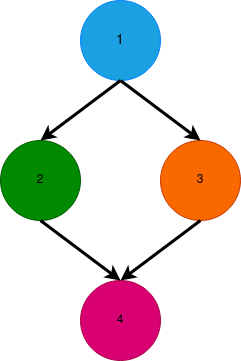
\includegraphics[scale=0.7]{Figures/reuse_example_graph.png}
\decoRule
\caption[reuseGraph]{Example of a graph with data reuse}
\label{fig:reuseGraph}
\end{figure}

Consider the computational graph of in figure \ref{fig:reuseGraph}. The graph clearly shows that
node 1's output will be reused as inputs to node 2 and 3. In a single SPM case,
we can see how the tensors would be mapped for each timestep. Clearly, the
leftover space of the SPM is what we can use as leftover pinning space between
operations. However, in the case of a multi-SPM architecture, this is not the
case as tensors cannot be split over different SPMs. To effectively navigate
the optimal mapping of pinned tensors, what SPM a tensor is pinned on greatly
affects the accumulated number of data transfers because of its effect on the
mapping of future tensors to an SPM. Once a tensor is pinned to a particular
SPM, mappings of inputs and outputs associated to other operations must be
remapped in accordance to the remaining capacity of all SPMs. This issue can be
compared to the bin-packing problem where the SPMs are bins and the tensors are
the items. Hence, for every possible mapping of a particular tensor to a SPM,
there exists new mapping for all other tensors that will exist for that
particular operation and future operations relative to the position of the
pinned tensor. The combinatorial explosion of possible mappings of tensors,
how long each one is mapped for, and where they are mapped is a search space
that grows with the depth of the deep learning model. An example of 
an un-optimal pinning strategy placing inputs and outputs without full consideration
of all future tensor placement combinations is shown in figure \ref{fig:pin_naive}.
In the figure, we can see that even though some tensors are able to be pinned,
there is unnecessary wasted space in some of the operations as well as other tensors
being written back and reloaded. Figure \ref{fig:pin_optimal} shows how a different
combination of tensor placements yields more reuse and less write backs to main
memory.

Notably, the single SPM case does not involve the concern of the exact location for
pinning a tensor. Rather, the decision making process in such a case is guided
solely by a tesnor's relative cost, its size, and the degree of overlap it has
with other tensors in terms of liveness. These factors shape how a pinned
tensor could influence future pinning opportunities for other tensors.
Due to these new considerations, simply porting the OnSRAM greedy algorithm 
leads to inefficient results since only a single scratchpad in the DLA can
be used for pinning.

Rather than porting the OnSRAM approach; a naively greedy approach in the
context of multiple SPMs has also been considered, i.e., initially pinning an
item to whatever SPM has the most space and remapping the inputs and outputs
accordingly. This process involves pinning outputs of every operation and
evicting the tensors when the pinned tensor cannot accommodate all other
necessary tensors for an operation, or when the output of the present operation
is of higher importance. The initial decision of selecting an SPM to pin an
item, which depends on the primary remapping of inputs and outputs around a
pinned tensor, can considerably influence the pinnability of future items. This
might, in certain instances, lead to the unpinned state of items immediately
prior to their reuse.

In such an approach, the system may not adequately identify opportunities for
reuse, leading to unpredictable decision-making and near-suboptimal results.
This limitation persists, albeit in a reduced form, even when the size of the
SPMs are increased. Therefore, to devise an algorithm that meticulously analyzes
possible decisions and maps tensors in a manner that effectively encourages
reuse, one could implement techniques such as graph coloring or ILP, which are
similar to the methods used in solving the pseudo-register SPM register
allocation problem.

Choosing an optimal pinning strategy to minimize the amount of data transfers
within this search space is the goal of this work.


\begin{figure}[th]
\centering
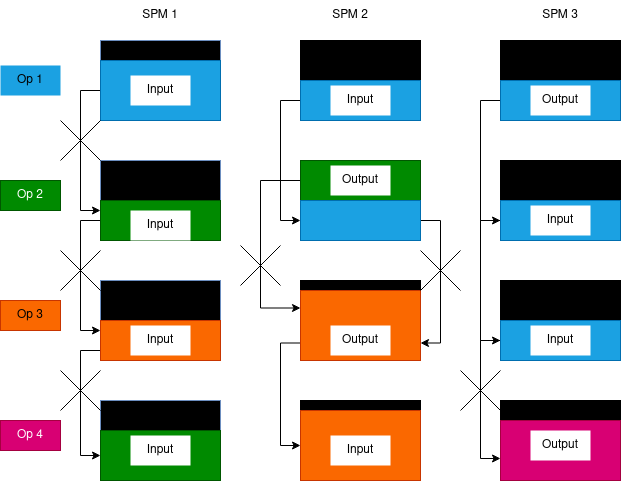
\includegraphics[scale=0.7]{Figures/reuse_example_pin_map_fail_1.png}
\decoRule
\caption[pin_naive]{Example of a un-optimal pinning strategy. Arrows
denote being pinned to the SPM and the crosses denote
an SPM being evicted due to capacity constraints.
Black denotes unused memory.}
\label{fig:pin_naive}
\end{figure}


\begin{figure}[th]
\centering
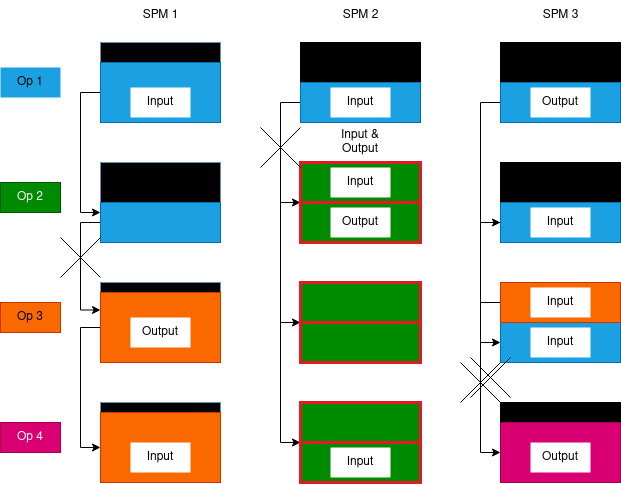
\includegraphics[scale=0.7]{Figures/reuse_example_pin_all.png}
\decoRule
\caption[pin_optimal]{Example of an optimal pinning strategy. Arrows
denote being pinned to the SPM and the crosses denote
an SPM being evicted due to capacity constraints. Red borders signify
distinction between different tensors created from the same operation.
Black denotes unused memory.}
\label{fig:pin_optimal}
\end{figure}
% we do everything in the 3 spm case
% goal is to mitigate data transfers between SPMs and main memory
% In order to analyze the possible mapping

\subsection{ILP based Multi-Scratchpad Allocation Strategy}
In order to analyze the search space and create a pin mapping for all tensors
such that the number of data transfers between SPMs and main memory on an
inter-node graph level are minimized, we propose an ILP model to create an
optimal strategy for a multi-scratchpad architecture.

To do this we first take an optimized computational graph and create a final
schedule of operators that will be ran. Using this schedule of operators, we
then aggregate all tensors that are used in the DNN. Each input and output
tensor is annotated with the operator from which it was created and all
operators that require it as a dependency. All tensor sizes, number of SPMs,
and the size of the SPMs are gathered as well. Using this information an
initial naive mapping scheme can be created where all inputs and outputs are
mapped to a designated input SPM and output SPM. All outputs are assumed to be
saved back to memory and reloaded when needed. We then use the initial mapping
as an input into the ILP solver to realize the optimal strategy.
 
%% Chapter Template

\chapter{Implementation} % Main chapter title

\label{Chapter5} % Change X to a consecutive number; for referencing this chapter elsewhere, use \ref{ChapterX}
%----------------------------------------------------------------------------------------
%	SECTION 1
%----------------------------------------------------------------------------------------
\section{Static Graph Analysis}
\subsection{SMAUG}

We first describe the simulation and compiler framework we work with in order
to show how tensors and mappings are obtained. SMAUG \cite{smaug} is an end to
end full stack simulation framework for deep learning work loads. As an
end-to-end framework SMAUG allows for a high level DSL to be used in order to
describe a model so that many deep learning architectures can be evaluated very
quickly. Further, SMAUG leverages the gem5-Aladdin \cite{aladdin} simulation
framework to describe custom hardware architectures, easily change their
configurations, all without the need for a dedicated backend compiler for each
custom architecture. This allows researchers to iterate and evaluate on many
deep learning workloads, and tune every layer of the stack without the need for
RTL design and laborious backed integrations. To the best of our knowledge, no
other simulation framework allows for the accurate performance analysis and
provides end-to-end configuration support.
\begin{figure}[thb!]
\centering
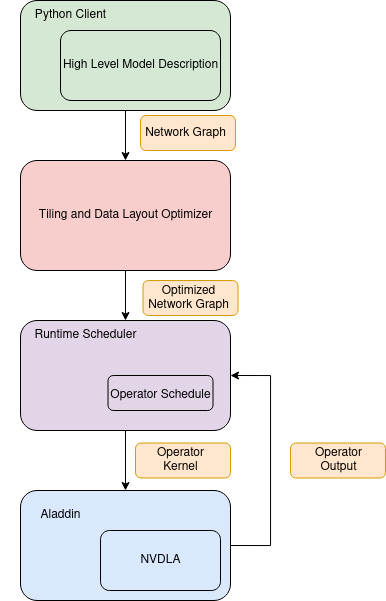
\includegraphics[scale=0.7]{Figures/smaug_stack.png}
\decoRule
\caption[Overview of SMAUG]{Overview of SMAUG framework stack}
\label{fig:SmaugStack}
\end{figure}


From SMAUG we can understand the amount of time and cycles being spent on compute time
over DMA transfers. Different deep learning models call for different operators that
result in diverse levels of memory and compute boundedness. Being able to
analyze operator level differences in DMA and compute times allow us to weight tensors
more heavily towards memory bound operations in the final ILP model.

\lstinputlisting[language=Python, caption={Model
description example},label={lst:minerva_model_desc}, basicstyle=\ttfamily\scriptsize]{Figures/minerva_network.py}


SMAUG is divided into a Python front end used to describe DL topologies, a
runtime middle end that handles execution, and a backend of kernels. An overview
of these parts are shown in figure \ref{fig:SmaugStack}. Models are
created using Python APIs that describe what operations, hardware
configuration, weights and input data, and which set of acerbated kernels a
user wants to use. The front end takes this model description and serialized it
into a form the runtime can read and create an execution context around. The
runtime takes the serialized model description and creates a computation graph.
Example code of a Minerva model description for SMAUG is show in listing
\ref{lst:minerva_model_desc}. The graph is used to perform tiling
optimizations and an operator schedule. Once an operator schedule is created,
the runtime executes each operation sequentially by dispatching each operation
as previous operator outputs are received back into main memory. The backend
contains all the accelerator kernels and are invoked every time the runtime
dispatches an operator. Kernels can be either written in native gem5 or using
Aladdin.
% TODO: figure of framework stack
% TODO: figure of a model description

% TODO: explain how backends are invoked and how hardware is described and configured
% TODO: explain the pipeline of tracing -> simulation for data gathering

\subsection{Static Analysis}

\begin{figure}[thb!]
\centering
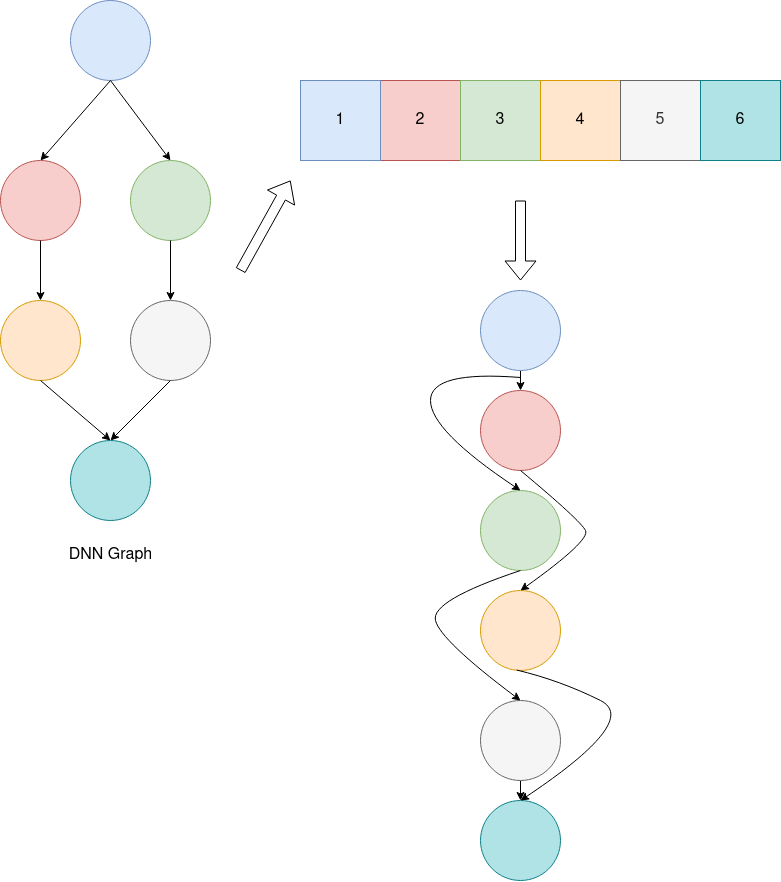
\includegraphics[scale=0.6]{Figures/graph_to_schedule.png}
\decoRule
\caption[Computational Graph to Schedule Conversion]{Illustration of a DNN graph being converted to a schedule}
\label{fig:graphToSchedule}
\end{figure}

Like OnSRAM, we use the computational graph provided by the SMAUG runtime
implemented in C++ to run our static analysis on tensors to devise a SPM
management framework. We allow SMAUG to apply its optimizations and graph
preprocessing to create a final operator schedule. This schedule is what we use
to analyze operator data dependencies and tensor meta information.  Figure
\ref{fig:graphToSchedule} shows how a DNN graph is converted into a schedule
where each node has a sequence number in the schedule. The schedule can be
visualized a new graph where nodes flow down sequentially in schedule order and
vertices show data dependencies. In SMAUG, each operation is represented as a
class has a list of associated input tensors, a list of output tensors, and
what computation the operation requires.  Each tensor is also represented as a
class that holds relevant information such as tensor size, dimensions, and
dimension layout.


% dict of inputs nad outputs per op for a scheudle list enumerate operations in
% the scheudle and create a mapping of a paritcular operation to the sequence
% number in the execution schedule

% create list of unique tensors
% create map of unique tensor to a unique tensor #

% create list of tensor size indexed by tensor #

% create map of tensor # to opreations sequence #'s its used in. The first element is the 
% operation # in which it is created and the last operation # is the final operation it is used in

We iterate through the schedule of operators and create a map where an
operation name is mapped to its sequence number in the operator schedule
For each operator we encounter for each iteration
of the schedule, we take note of the operators input and output tensors. These inputs
and outputs are used to create an array of unique tensors. This array of
tensors is then used to create a mapping of each tensor to a tensor number
where every tensor number is the index of the tensor in the array. A map of 
tensor numbers to the corresponding tensor size is also created. We then
build a map of tensor numbers to an array of operation sequence numbers they are
required in where the first element of the array represents the operation that
the tensor is created and the last element represents the final operation
it is used in.

%TODO: figure of graph -> operator schedule -> data reuse graph



\begin{figure}[thb!]
\centering
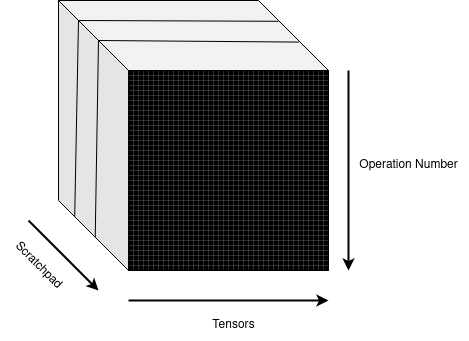
\includegraphics[scale=0.7]{Figures/mapping_matrix_cube.png}
\decoRule
\caption[3D Tensor Mapping Matrix]{Illustration of mapping matrix}
\label{fig:mappingCube}
\end{figure}


\begin{figure}[thb!]
\centering
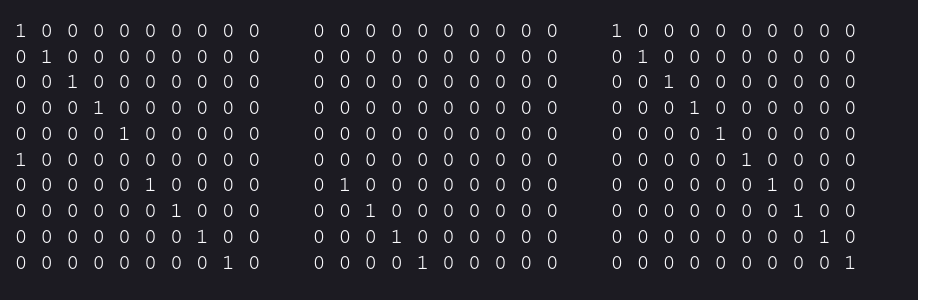
\includegraphics[scale=0.5]{Figures/naive_matrix_mapping.png}
\decoRule
\caption[2D Tensor Mapping Matrix]{Naive SPM mapping matrix representation as an input to the ILP solver}
\label{fig:naiveSPM2D}
\end{figure}

\subsection{SPM Mapping Representation}

The way an SPM mapping is represented is a three dimensional array in which one
dimension represents time i.e the operation sequence number, another represents
the unique tensors, and the final dimension represents what scratchpad they
belong to. Using the dimensions we can show the relationship between what tensor
is mapped to what SPM during what operation. We build such a matrix after the
static analysis phase to formulate an initial naive SPM mapping representation
that would be executed by default on SMAUG. Figure \ref{fig:naiveSPM2D}
illustrates in two dimensions the resulting naive SPM mapping matrix.

% TODO: remake the matrix cube where we blow up a element to show a tensor and
% like a mapping to the grpah or something
%----------------------------------------------------------------------------------------
%	SECTION 2
%----------------------------------------------------------------------------------------
\section{Model Formulation}

We now describe our ILP model to solve the SPM mapping optimization problem. The goal is to minimize
the amount of cost weighted data transfers as much as possible by pinning as many re-usable tensors
as possible. As described in the previous section, we can breakdown a DNN graph into the following variables.

% describe how we structure our matrix
% data trasnfers costs are proportional the size of the tensor being transported because of the limited bandwidth of hte bus, therefore
% tensors with larger sizes will be weighted as a higher cost. The overall transfer itself can be modelled as data entering the SPM and being
% offloaded from the SPM to main memory. This is done by represneting whether a tensor is on teh SPM with a binary variable: 0 for the tensor is in main
% memory and 1 to represnte hte tensor is in the SPM. A tensor being loaded into the SPM from main memory is modelled as a 0 to 1 in the tenosr column. 
% A tensor being saved to main memory is modelled as 1 to 0 in teh tensor time column x[m][k][n] = 1 x[m+1][k][n] = 0

There exists a set of tensors required as inputs and outputs per operation and a unique list of tensors can be constructed.\\
\\
Let $N \coloneqq \{ n \text{ }  | \text{ } n   \text{ represents a tensor ID used in the DNN graph}\}$\\

For each DLA architecture, there exists at least 1 scratchpad with a corresponding size. To refer to each scratchpad and its size on the DLA:\\
\\
Let $K \coloneqq \{ k \text{ }  | \text{ } k   \text{ represents a scratchpad ID}\}$\\
Let $Q \coloneqq \{ q \text{ }| \text{ } \text{where } Q_k \text{ represents the size of Scratchpad$_k \in K$}\}$\\

Once a graph has been scheduled, each operation can be referenced by its sequence number.\\
\\
Let $M \coloneqq \{ m \text{ }  | \text{ } m   \text{ represents an operation in the DNN graph}\}$\\

Due to limited bus bandwidth, tensors with different sizes will require
different amounts of DMA transfers proportional to their size. In order to keep
track of the sizes so that we can weight each tensor with a certain cost:\\
\\
Let $S \coloneqq \{ s \text{ }| \text{ } \text{where } S_n \text{ represents the size of tensor$_n \in N$}\}$\\


So the mapping matrix can be described as a three dimensional matrix where every position is a binary variable such that\\
\\
$x[n][k][m] \in \{0, 1\} \forall n,k,m $\\
$x[n][k][m] = 1$ represents a tensor $n$ that occupies scratchpad $k$ at operation $m$ \\
$x[n][k][m] = 0$ represents a tensor $n$ does not exist on scratchpad $k$ at operation $m$\\

If $x[n][k][m] = 0 \forall k$ then it means that tensor $n$ is saved to main memory at operation $m$.


\subsection{Objective Function}
The objective function we would like to solve for such that we minimize the
amount of cost weighted data transfers is the following:\\
\\
\[
min(\sum_n \sum_k \sum_m S_n * (|x[n][k][m+1] - x[n][k][m]|))
\]
\\

A difference between $|x[n][k][m+1] - x[n][k][m]|$ represents either a data
transfer of tensor $n$ from SPM $k$ to main memory if $x[n][k][m+1] -
x[n][k][m] = -1$ or main memory to SPM if $x[n][k][m+1] - x[n][k][m] = 1$.
$|x[n][k][m+1] - x[n][k][m]|$ shows that either a tensor $n$ remains on SPM $k$
between operations $m$ and $m+1$ or stays in main memory.

By minimizing the sum of total data transfers multiplied by the tensor size, we
minimize on a cost basis the amount of DMA loads and stores and maximize
tensors being reused on the SPM. However, the absolute value in the objective function
would make it non-linear. Thus, we add auxiliary variables to remove the absolute values
and reformulate the objective function as:\\
\\
\[
min(\sum_n \sum_k \sum_m y[n][k][m])
\]

\subsection{Constraints}
We now describe the following set of constraints on the model:
\begin{itemize}
	\item All necessary input and output tensors for a given operation will be present on the SPMs\\

		Let $A \coloneqq \{ a \text{ } | \text{ } \text{where } A[n] = 1\text{ represents a tensor$_n$ is required as an input or output for operation$_m$} \}$\\
		\[
			A[n][m] \in \{0, 1\} \forall n,m
		\]

		\[
			A[n][m] = 1 \implies \sum_{i \in K} x[n][i][m] = 1 
		\]

	\item All tensors mapped on an SPM$_k$ must fit on within the given scratchpad space\\

		$\sum_{i \in N} {x[i][k][m] * s[i]} \leq Q[k] \forall m,k$\\

	\item Tensors are not mapped before the operation in which they're lifetime begins \\

		Let $B \coloneqq \{ b_n \text{ } | \text{ }  b_n \text{represents the start time for tensor $n$}\}$ \\

		$x[n][m][k] = 0 \forall m < B_m$

	\item Tensors are not mapped after the operation in which they're lifetime ends \\

		Let $E \coloneqq \{ e_n \text{ } | \text{ }  e_n \text{represents time for tensor $n$}\}$ \\

		$x[n][m][k]= 0 \forall m > E_m$

	\item Absolute Value Constraints\\
		Let $Y = \{ y[0][0][0], y[0][0][1], ... y[n][k][m]\prime\}$\\
		$(x[n][k][m+1] - x[n][k][m]) * S_n <= y[n][k][m]$\\
		$(x[n][k][m] - x[n][k][m + 1]) * S_n <= y[n][k][m]$\\

\end{itemize}

\subsection{Solver}
This model description can now be used to find the exact solution to the SPM
mapping problem. We use the Gurobi ILP solver and the Python API to create our
optimized mapping matrix. The listed constraints can be used as is and the
original $X$ variable is initialized with the naive mapping matrix.  An
illustration of the optimized matrix is show in figure \ref{fig:optimalSPM2D}.
This new matrix can be used to integrate a pinning strategy in the framework.

\begin{figure}[thb!]
\centering
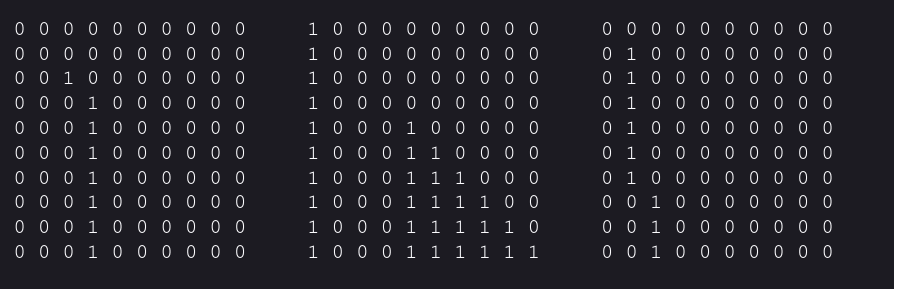
\includegraphics[scale=0.55]{Figures/optimal_matrix_mapping.png}
\decoRule
\caption[Optimal Mapping 2D Matrix]{Optimal SPM mapping matrix representation as an input to the ILP solver}
\label{fig:optimalSPM2D}
\end{figure}

 

%----------------------------------------------------------------------------------------
%	THESIS CONTENT - APPENDICES
%----------------------------------------------------------------------------------------

\appendix % Cue to tell LaTeX that the following "chapters" are Appendices

% Include the appendices of the thesis as separate files from the Appendices folder
% Uncomment the lines as you write the Appendices

% Appendix A

\chapter{Frequently Asked Questions} % Main appendix title

\label{AppendixA} % For referencing this appendix elsewhere, use \ref{AppendixA}

\section{How do I change the colors of links?}

The color of links can be changed to your liking using:

{\small\verb!\hypersetup{urlcolor=red}!}, or

{\small\verb!\hypersetup{citecolor=green}!}, or

{\small\verb!\hypersetup{allcolor=blue}!}.

\noindent If you want to completely hide the links, you can use:

{\small\verb!\hypersetup{allcolors=.}!}, or even better: 

{\small\verb!\hypersetup{hidelinks}!}.

\noindent If you want to have obvious links in the PDF but not the printed text, use:

{\small\verb!\hypersetup{colorlinks=false}!}.


%\include{Appendices/AppendixB}
%\include{Appendices/AppendixC}

%----------------------------------------------------------------------------------------
%	BIBLIOGRAPHY
%----------------------------------------------------------------------------------------

\printbibliography[heading=bibintoc]

%----------------------------------------------------------------------------------------

\end{document}  

